\chapter{WWW視覚化}
\label{chap:visualize}

この章ではではDreamSacpeがiOSアプリで睡眠中に音を流すという形に至った背景を述べる。

\section{音に着目した背景:夢を効果的に操作するインプットについて調査}
\subsection{実験:香りをインプットとして作ったプロトタイプ}
実験内容:5日間非常に親しくしている友人人がいつも部屋で使っているアロマオイルをつけて寝ることでその人との思い出やその部屋での思い出を夢で見ることができないかを実験。しかし5日中それに関連した夢を見ることはできなかった。効果があまり出なかったのは睡眠中嗅覚はあまり機能していないためであると考えられる。
\begin{figure}[htbp]
\begin{center}
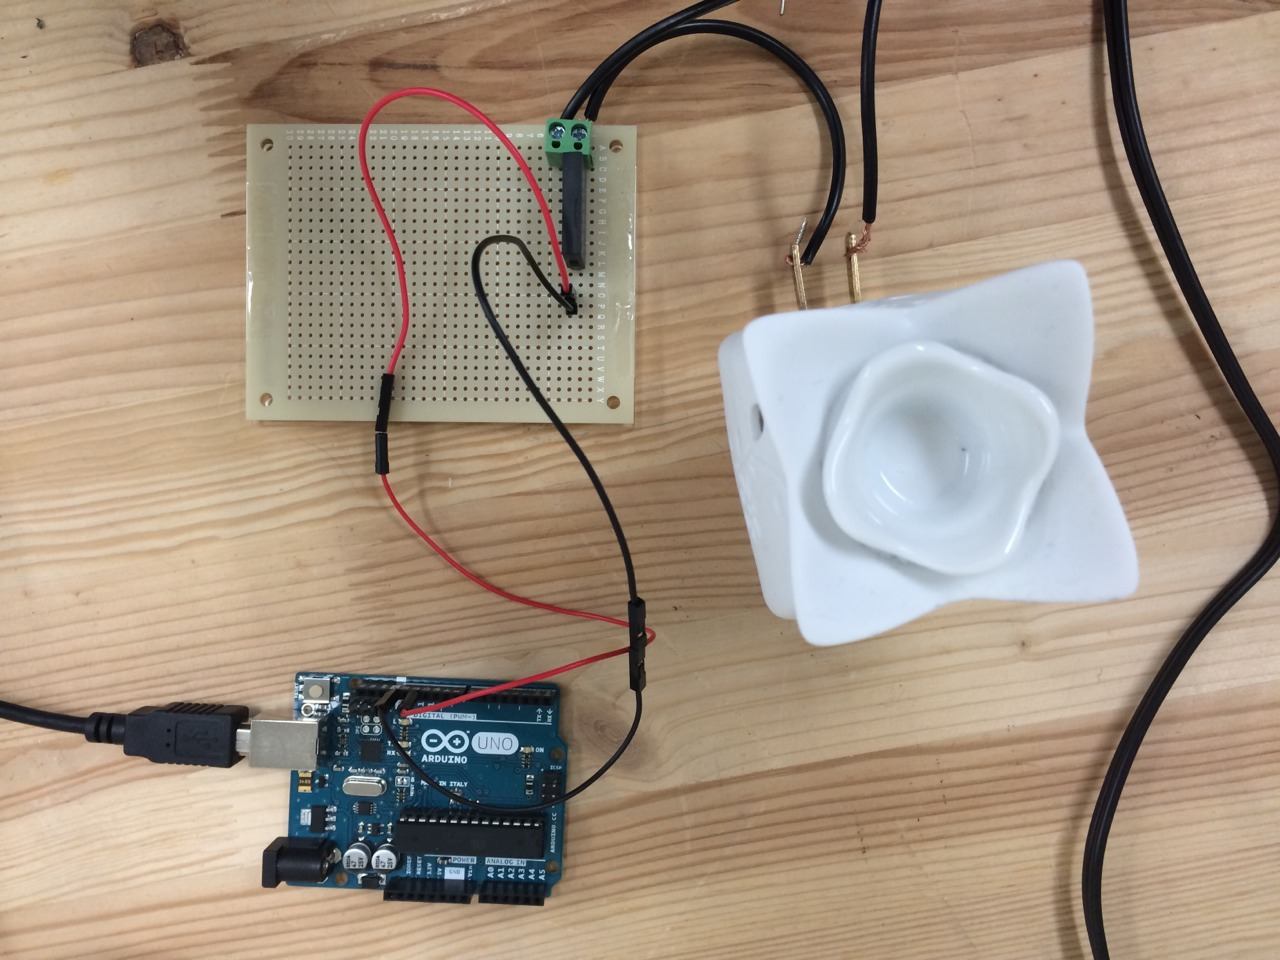
\includegraphics[width=15cm]{eps/smell.eps}
\caption{匂いによるインプット}
\label{匂いによるインプット}
\end{center}
\end{figure}

\subsection{実験:音をインプットとして作ったもの}
実験内容:5日間上で述べた同じ友人と一緒に聞いた音楽を流しならが寝たところ、5日に2日その人に関連した夢を見た。よって香りより音による刺激脳が夢に影響を与えやすいということが分かった。


\section{iOSアプリに至った背景:REM睡眠のセンシング方法}
\subsection{実験1:kinect}
特徴:精度が低い、価格が高い、取り付けに労力が必要とされる、ポータブルではないため旅先では使えない
\begin{figure}[htbp]
\begin{center}
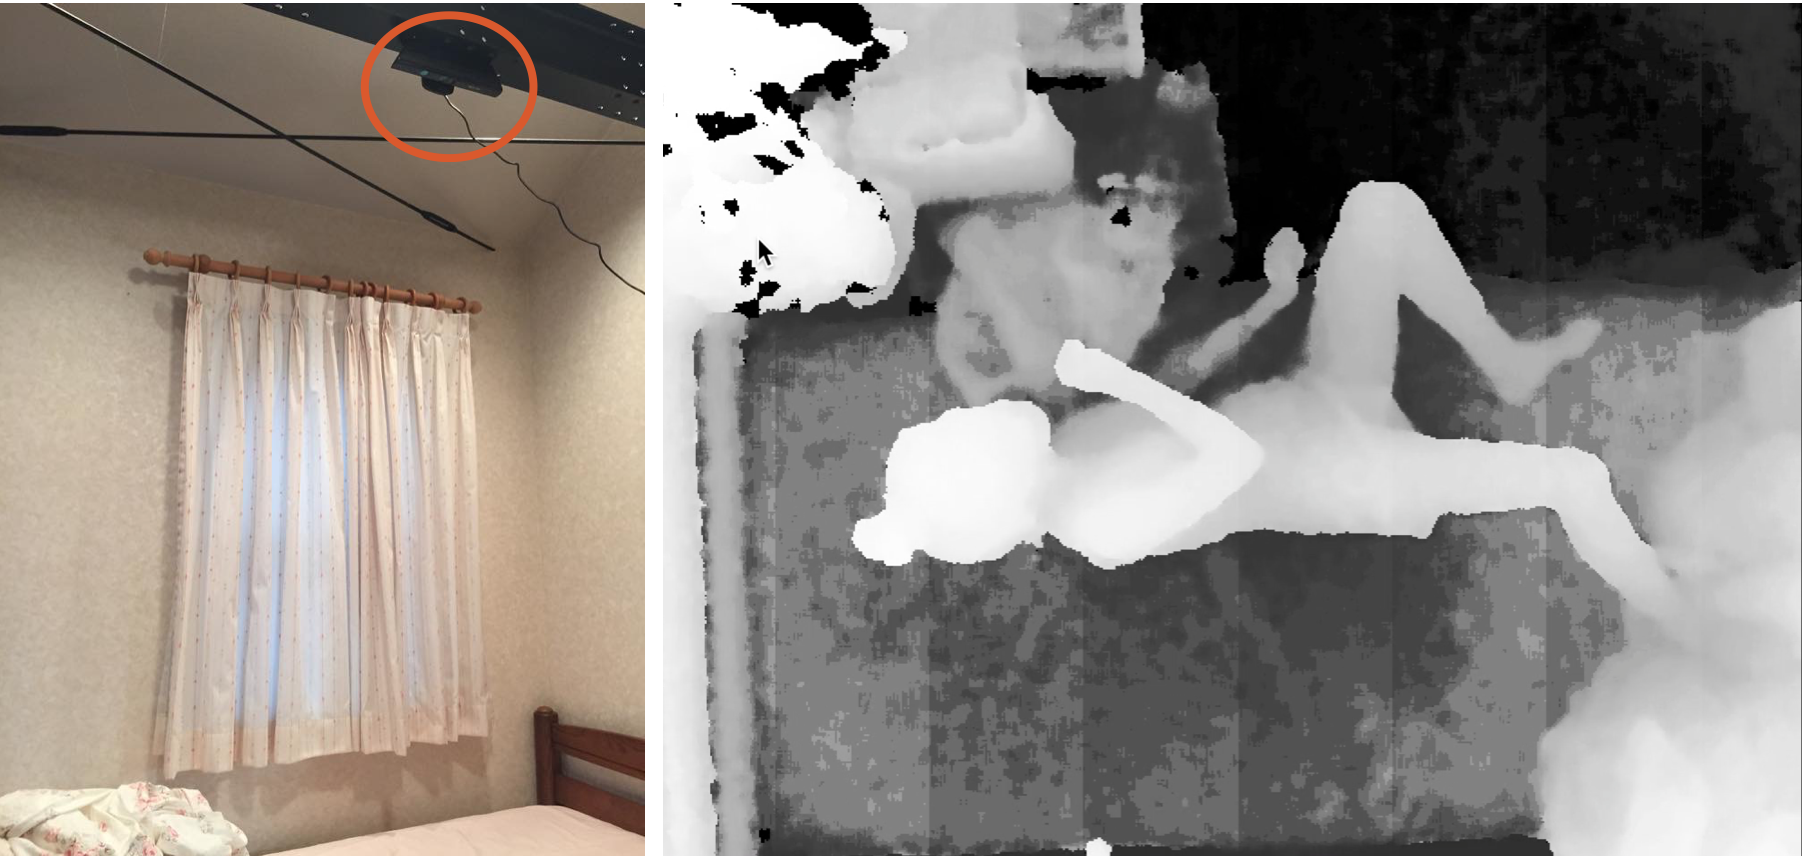
\includegraphics[width=15cm]{eps/kinect.eps}
\caption{kinectによるモニタリング}
\label{kinectによるモニタリング}
\end{center}
\end{figure}

\subsection{実験2:mindWave}
特徴:締め付けられる感覚があり、且つ汗をかいてしまうのでユーザーに負担がかかる、正確である
\subsection{実験3:パルスセンサー}
特徴:身につけていないといけない
\subsection{実験4:iOSアプリ}
特徴:ウェラブルではないため身軽、iOSのスマートフォンを持っている人であれば、大人数の人に比較的簡単に使ってもらえる、安全である、余計な費用がかからない、持ち運びが簡単なので旅中も使える
